\section{低质量区间}

在低质量区间中,双电子的额外产额谱主要由受介质影响的$\rho$介子质量谱和来自于夸克胶子等离子体热辐射的双电子两部分构成,其中占最主要的部分是受介质影响的$\rho$介子质量谱。

图\ref{fig:Hm_ExY_LMR_54GeV_27GeV_NA60_RhoAndQGPfit_icent0}为STAR实验中 \sNN = 54.4 GeV, \sNN = 27 GeV 金-金对撞以及NA60实验中\sNN = 17.3 GeV铟-铟对撞中低质量区间双轻子额外产额比较\cite{Specht:2010xu}。其中STAR的测量为0-80\%中心度当中的测量结果,NA60的结果在$\rm{dN_{ch}/dy > 30}$的中心度区间内。
为了去掉volume effect的影响,STAR中的双轻子额外产额谱均进行了对于$dN_{ch}/dy$的归一化,从而和NA60实验中\sNN = 17.3 GeV铟-铟对撞中经过归一化处理的双轻子额外产额进行比较。

可以看到在$\rho$为主要来源的质量区间(低质量区间),STAR的双电子额外产额谱测量结果和NA60的结果符合得很好。在这个质量区间当中,受介质影响的$\rho$介子质量谱可以由一个Breit-Wigner(BW)分布再乘上Boltzmann因子(PS)来描述,具体形式见式\ref{eq:rho_spectra}\cite{STAR:2002caw,Shuryak:2002kd,Kolb:2003bk,Rapp:2003ar}。其中 $\Gamma$的具体形式见式\ref{eq:BW}。当$\rm{M_{ee} \ll M_0}$时,式\ref{eq:BW}可近似为$\Gamma_0~*~\frac{M_0}{M_{ee}}$的形式。其中$\Gamma_0~$和$M_0$分别为$\rho$的静质量。Boltzmann因子的具体形式为\ref{eq:PS}所示。其中 $T_{med}$为介质的温度。

除了 $\rho$的贡献以外,在这个质量区间内双电子谱还有一部分来源于夸克胶子等离子体的热辐射的双电子。这一部分由式\ref{eq:QGP_thermal}\cite{Rapp:2014hha}所描述。

在拟合当中为了描述 $\rho$ 和 热辐射两者对双电子额外产额谱的贡献,使用一个由式\ref{eq:rho_spectra}和式\ref{eq:QGP_thermal}相加得到的方程来对额外产额谱进行拟合。就可以抽取在这个区间当中的介质的温度。图\ref{fig:Hm_ExY_LMR_54GeV_27GeV_NA60_RhoAndQGPfit_icent0}中列出了对三组实验结果的拟合结果,STAR \sNN = 54.4 GeV金-金对撞中其他中心度的拟合结果列在表\ref{tab:T_fitting_result_LMR}当中。

可以看到在不同的对撞系统(铟-铟和金-金)以及不同的对撞能量(\sNN = 17.3, 27, 54.4 GeV)下,双电子额外产额谱的形状类似并且拟合所抽取得到的温度结果都比较接近。且在误差范围内都与格点量子色动力学计算得到的的相变温度 $\rm{T_{pc} = 154 MeV}$\cite{HotQCD:2018pds}相符合,这就意味着 $\rho$ 很可能产生在发生相变的阶段附近。

\begin{equation}
    \label{eq:rho_spectra}
    M_{ee}^{\rho} = a*BW*PS
\end{equation}
\begin{equation}
    \label{eq:BW}
    \begin{split}
        BW =\frac{M_{ee}M_{0}\Gamma}{[(M_0^2-M_{ee}^2)^2+M_0^2\Gamma_0^2]}\\
        \Gamma = \Gamma_0~*~\frac{M_0}{M_{ee}}~*~\frac{M^2_{ee}-4M_e^2}{M_0^2-4Me^2}^{3/2}
    \end{split}
\end{equation}
\begin{equation}
    \label{eq:PS}
    PS = e^{-M_{ee}/T_{med}}
\end{equation}
\begin{equation}
    \label{eq:QGP_thermal}
    M_{ee}^{QGP} = M_{ee}^{3/2}~*~PS
\end{equation}

\begin{figure}[htb]
    \begin{center}
    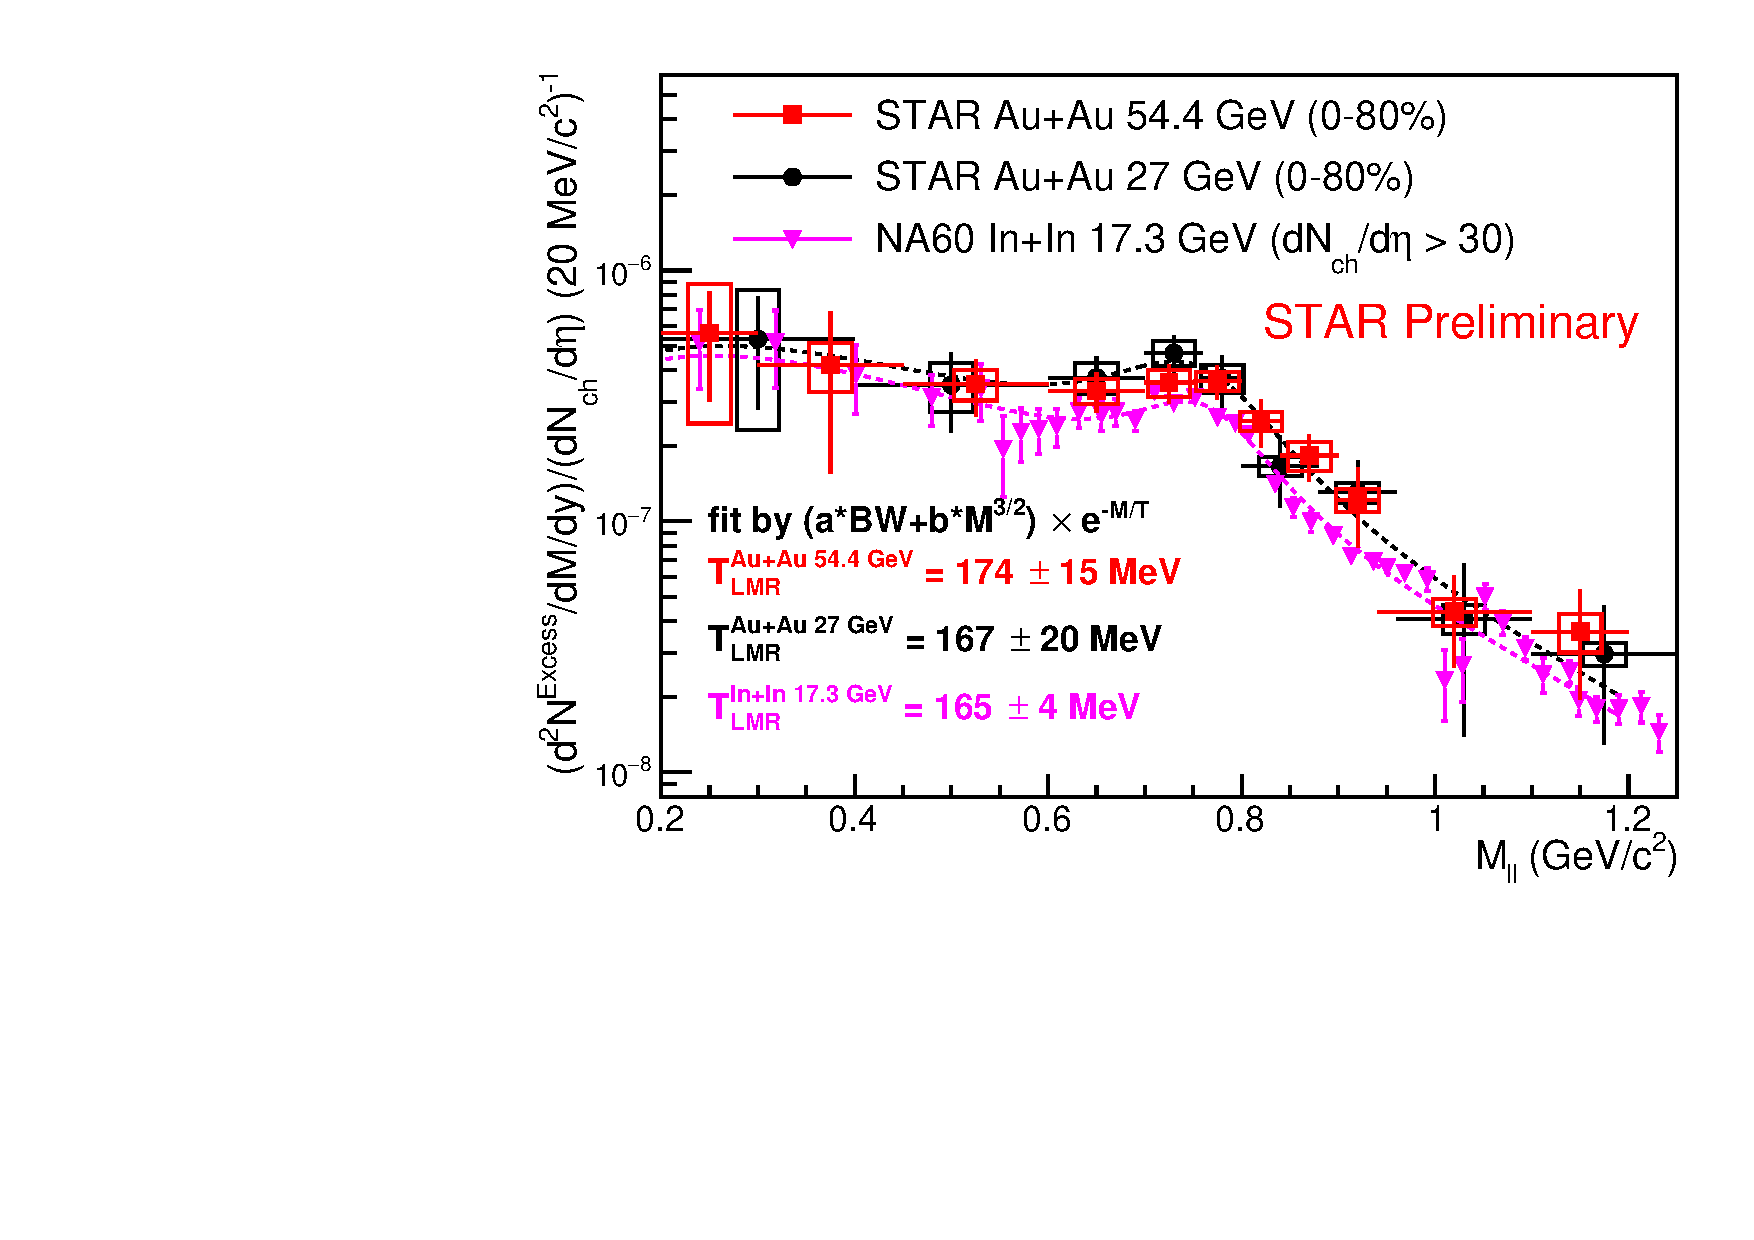
\includegraphics[width=0.75\textwidth,clip]{figures/Chapter4/Hm_ExY_LMR_54GeV_27GeV_NA60_RhoAndQGPfit_icent0.pdf}
    \end{center}
    \caption[STAR实验中 \sNN = 54.4 GeV, \sNN = 27 GeV 金-金对撞以及NA60实验中\sNN = 17.3 GeV铟-铟对撞低质量区间双轻子额外产额谱比较示意图]{STAR实验中 \sNN = 54.4 GeV, \sNN = 27 GeV 金-金对撞以及NA60实验中\sNN = 17.3 GeV铟-铟对撞中低质量区间双轻子额外产额比较,三个双轻子额外产额均用式进行拟合来抽取对撞温度信息。}
    \label{fig:Hm_ExY_LMR_54GeV_27GeV_NA60_RhoAndQGPfit_icent0}
\end{figure}

\begin{table}[h!]
    \centering
    \caption{54.4GeV金-金对撞低质量区间不同中心度通过拟合抽取得到的温度的结果}
    \label{tab:T_fitting_result_LMR}
    \begin{tabularx}{1\textwidth} {
    | >{\centering\arraybackslash}X |>{\centering\arraybackslash}X |>{\centering\arraybackslash}X |>{\centering\arraybackslash}X |>{\centering\arraybackslash}X | }
        \hline
        Centrality  & $T_{med}$ \\
        \hline
        0-80\%  & $175 \pm 15$   \\
        \hline
        0-10\%  & $182 \pm 31$ \\
        \hline
        10-40\% & $175 \pm 17$\\
        \hline
        40-80\% & $197 \pm 13$\\
        \hline
    \end{tabularx}
\end{table}

除了通过拟合来抽取介质的温度,双电子的额外产额谱也和两种理论模型的计算结果进行了比较,结果如图\ref{fig:Model_Compare}所示。两种模型分别为Rapp模型\cite{Rapp:2014hha, Rapp:2000pe, Rapp:2013nxa}和PHSD(Parton-Hadron-String Dynamics)模型\cite{Bratkovskaya:2007jk, Bratkovskaya:1996qe, Song:2018xca}。其中Rapp 模型使用宏观多体方法来描述介质的演化,PHSD模型通过微观输运的方法来描述介质的演化,在两个模型的计算中均包括了介质中$\rho$介子谱和夸克胶子等离子体热辐射的贡献。从图中可以看到和\sNN = 27 GeV的结果相比,Rapp和PHSD模型都可以很好的描述数据。当和\sNN = 54.4 GeV的结果相比时,Rapp 模型在$\rm{M_{ee} > 0.8~GeV/c^2}$的区间内可以很好的描述数据,但在$\rm{ 0.5 < M_{ee} < 0.8~GeV/c^2}$的区间内对数据有些高估。PHSD模型在$\rm{M_{ee} < 0.9~GeV/c^2}$的区间内对数据有些低估,在其他的质量区间内可以很好的描述数据。
\begin{figure}[htb]
    \centering
    \begin{subfigure}[b]{0.45\textwidth}
        \centering
        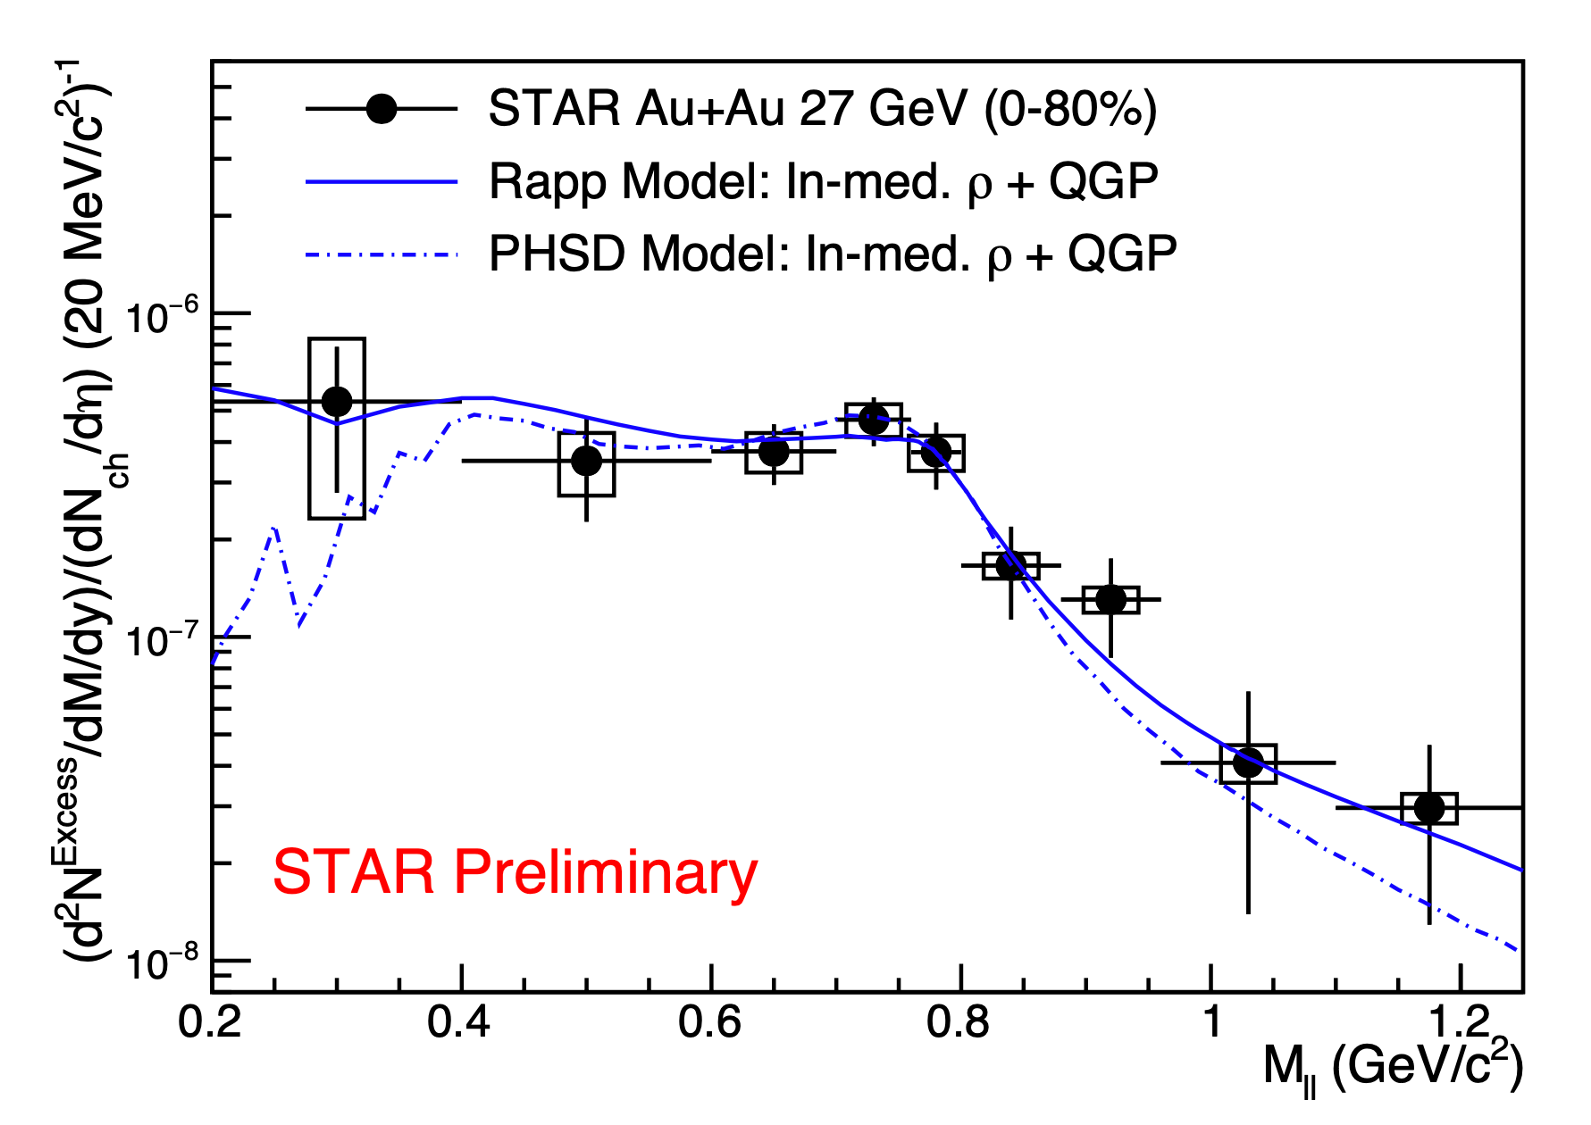
\includegraphics[width=\textwidth,clip]{figures/Chapter5/Model_Compare_27.png}
        \caption{}
        \label{fig:Model_Compare_27}
    \end{subfigure}
    \hfill
    \begin{subfigure}[b]{0.45\textwidth}
        \centering
        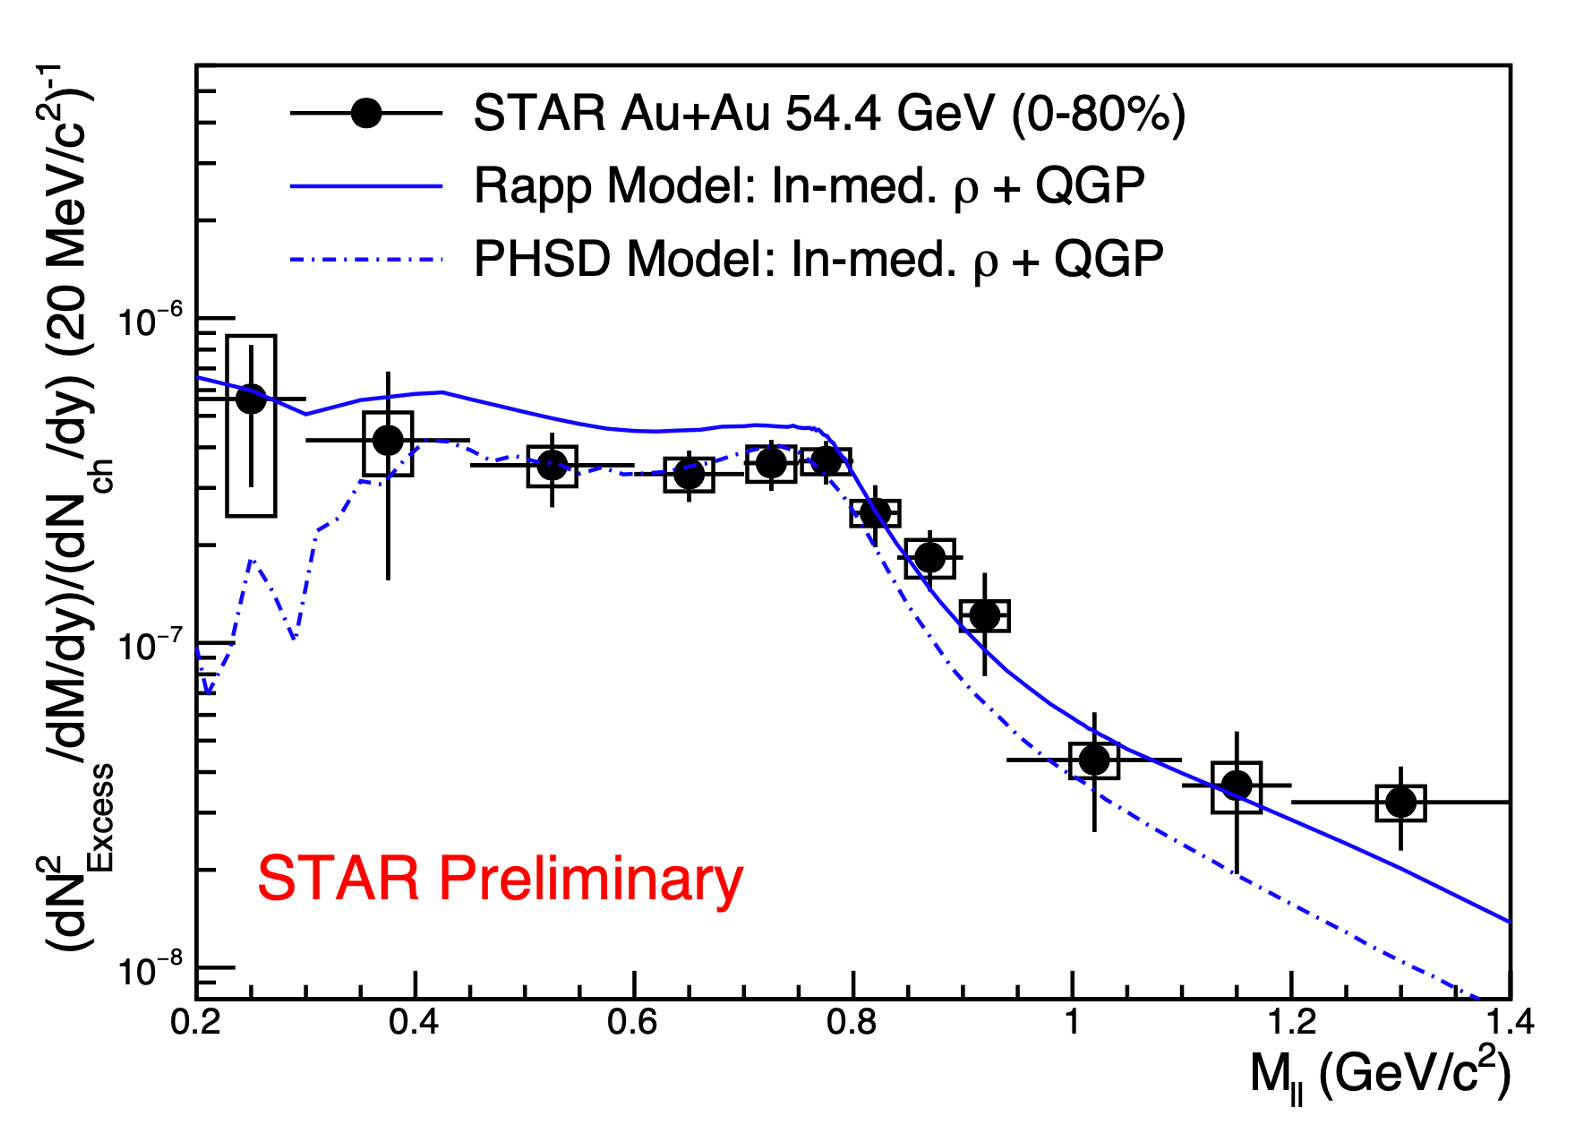
\includegraphics[width=\textwidth,clip]{figures/Chapter5/Model_Compare_54.png}
        \caption{}
        \label{fig:Model_Compare_54}
    \end{subfigure}
    \caption[0-80\%下\sNN = 54.4 GeV, \sNN = 27 GeV 金-金对撞中双电子额外产额谱和模型比较示意图]{0-80\%下\sNN = 54.4 GeV, \sNN = 27 GeV 金-金对撞中双电子额外产额谱和模型比较示意图,左图为\sNN = 27 GeV的结果,右图为\sNN = 54.4 GeV的结果。}
    \label{fig:Model_Compare}
\end{figure}

